\begin{figure}[h]
    \centering
    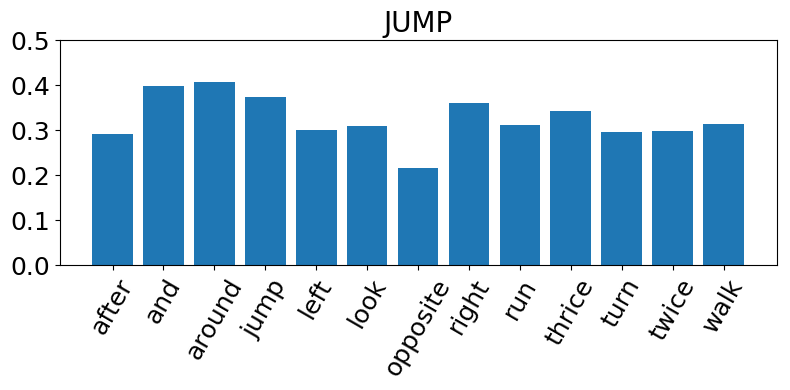
\includegraphics[width=.4\textwidth,keepaspectratio]{figures/jump_error_dist.png}
    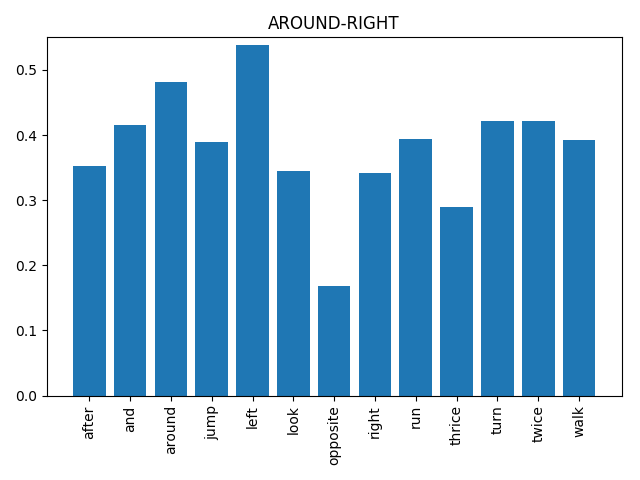
\includegraphics[width=.4\textwidth,keepaspectratio]{figures/template_error_dist.png}
    \caption{Proportion of commands with a certain word (over word
      total) that were wrongly executed by the respective best CNNs in
      the \emph{jump} (t) and \emph{template} (b) splits.}
    \label{fig:error_distributions}
\end{figure}


Although the CNNs dramatically outperform the RNNs, their performance
is still far from perfect (cf.~\label{table:main results}). The SCAN
tasks are designed to be easy for a system that has learned the right
composition rules. Perhaps, CNN's performance is not perfect because
they only learned a subset of the necessary rules. For example, they
might be able to correctly interpret the new expression \emph{jump
  twice} because they induced a \emph{X twice} rule from their
training set, but they might fail at \emph{jump thrice} because they
failed to learn the corresponding \emph{X thrice} rule. Since SCAN
semantic composition rules are associated with single words in input
commands, we can check this hypothesis by looking at error
distribution across input words. It turns out that, in neither the
\emph{jump} nor the \emph{around-split}, errors are strongly
associated to specific input commands. Figure
\ref{fig:error_distributions} shows proportion of errors in commands
containing a word (over total occurrences of the word) made by the
best models in each split. Besides observing that \emph{opposite} is
consistently easier, we observe a relatively stable proportion of
errors across command words (the hardest word, \emph{left} in the
\emph{around-right} split, is wrongly executed in 54\% of the cases in
which it occurs). Direct inspection of the errors reveals no traces of
systematicity. Indeed, we often find minimal pairs in which changing
one action verb with another (distributionally equivalent in SCAN)
turns a correctly executed command into one where the CNN fails. For
example, in the \emph{jump} split, the CNN correctly executes
``\emph{jump left after walk},'' but fails ``\emph{jump
  left after run}'' (jumping is forgotten). Analogously, in the
\emph{around-right} split, ``\emph{run around right}'' is correctly
executed, but ``\emph{walk around right}'' isn't (the CNN stops too
soon).
